\section{Implementazione}
\subsection{VanillaCase}
Nella seguente figura è possibile osservare le connessioni logiche tra tre FMU principali: 
\begin{itemize}
	\item \textbf{FMU of the leading car}: questa FMU implementa il comportamento della leading car. Per funzionare non ha bisogno di alcun input da altre FMU e produce in output la posizione della macchina, la velocità e la sua accelerazione. 
	\item \textbf{FMU of the following algorithm}: questa FMU implementa l'algoritmo di inseguimento. Presi in ingresso i parametri di posizione, velocità e accelerazione della leading car ed i parametri di posizione e velocità della following car produce in output l'accelerazione per la following car.
	\item \textbf{FMU of the following car}: questa FMU implementa il comportamento della following car. Per funzionare prende in ingresso l'accelerazione dalla precedente FMU e produce in output la sua posizione e velocità.
\end{itemize}
\begin{figure}[H]
	\centering
	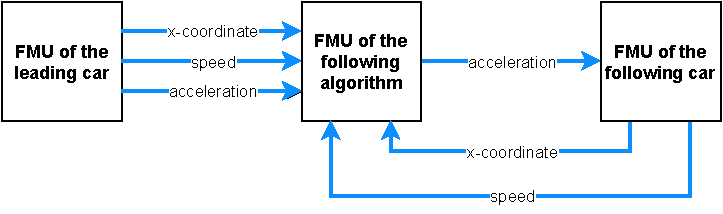
\includegraphics{img/VanillaSchema.pdf}
	\caption{Multi-Model schema del VanillaCase}
\end{figure}

In figura 2 viene rappresentata l'overview del relativo Multi-Model sviluppato con il tool INTO-CPS. 

\begin{figure}[H]
	\centering
	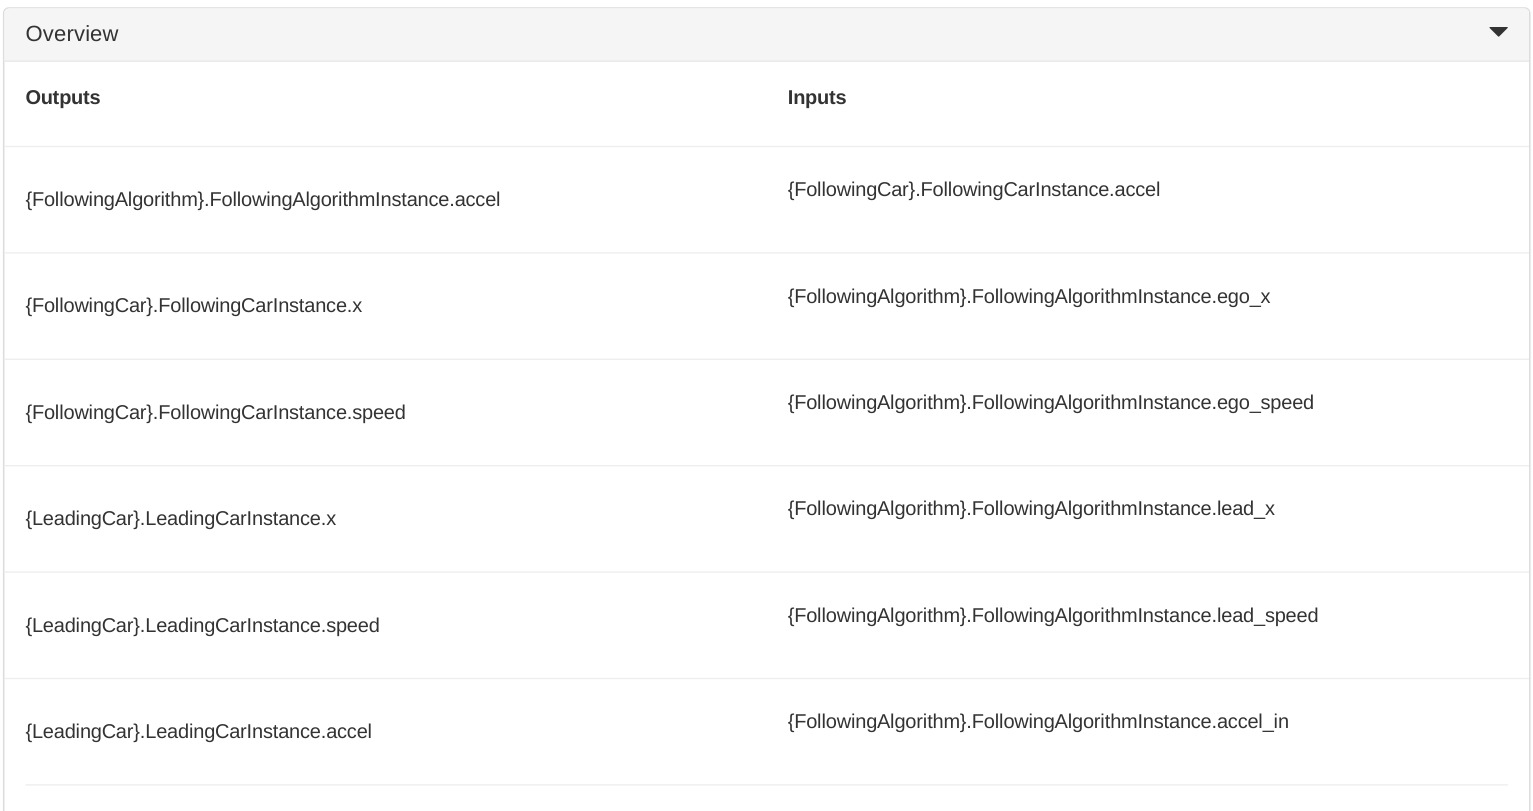
\includegraphics[width=\textwidth]{img/OverviewVanilla.png}
	\caption{Multi-Model Overview del Vanilla Case}
\end{figure}

\subsection{Attacco all'accelerazione}
A differenza dello schema presentato nel VanillaCase, viene ora aggiunta una ulteriore FMU situata fra "FMU of the following algorithm" e "FMU of the following car" già presenti. La nuova FMU implementa con strategia \textit{Man-in-the-Middle} un attacco di tipo data alteration sull'accelerazione passata tra il Following Algorithm e la Following Car. Fare riferimento alla sezione 3.5 per dettagli sul comportamento dell'attacco.
\begin{figure}[H]
	\centering
	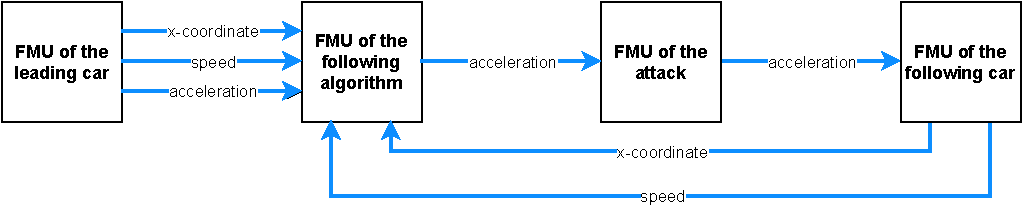
\includegraphics{img/AccelAttackSchema.pdf}
	\caption{Multi-Model schema dell'Attacco alla Accelerazione}
\end{figure}

In figura 4 e 5 viene rappresentata l'overview del relativo Multi-Model sviluppato con il tool INTO-CPS. 

\begin{figure}[H]
	\centering
	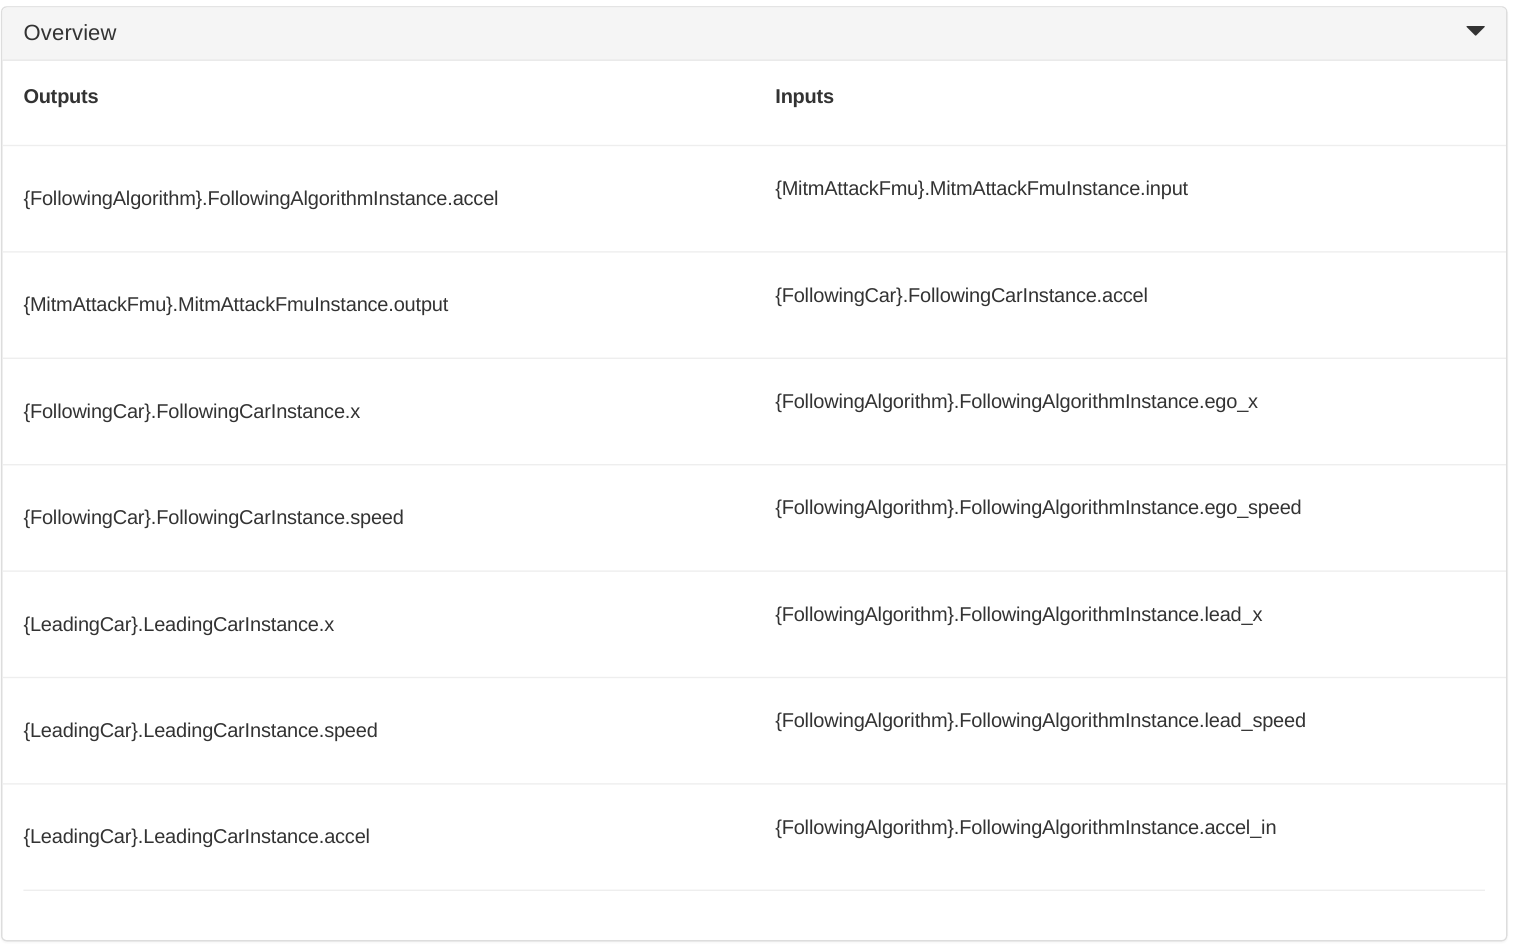
\includegraphics[width=\textwidth]{img/OverviewAccelSingle.png}
	\caption{Multi-Model Overview dell'attacco all'accelerazione (caso attacco semplice)}
\end{figure}
\begin{figure}[H]
	\centering
	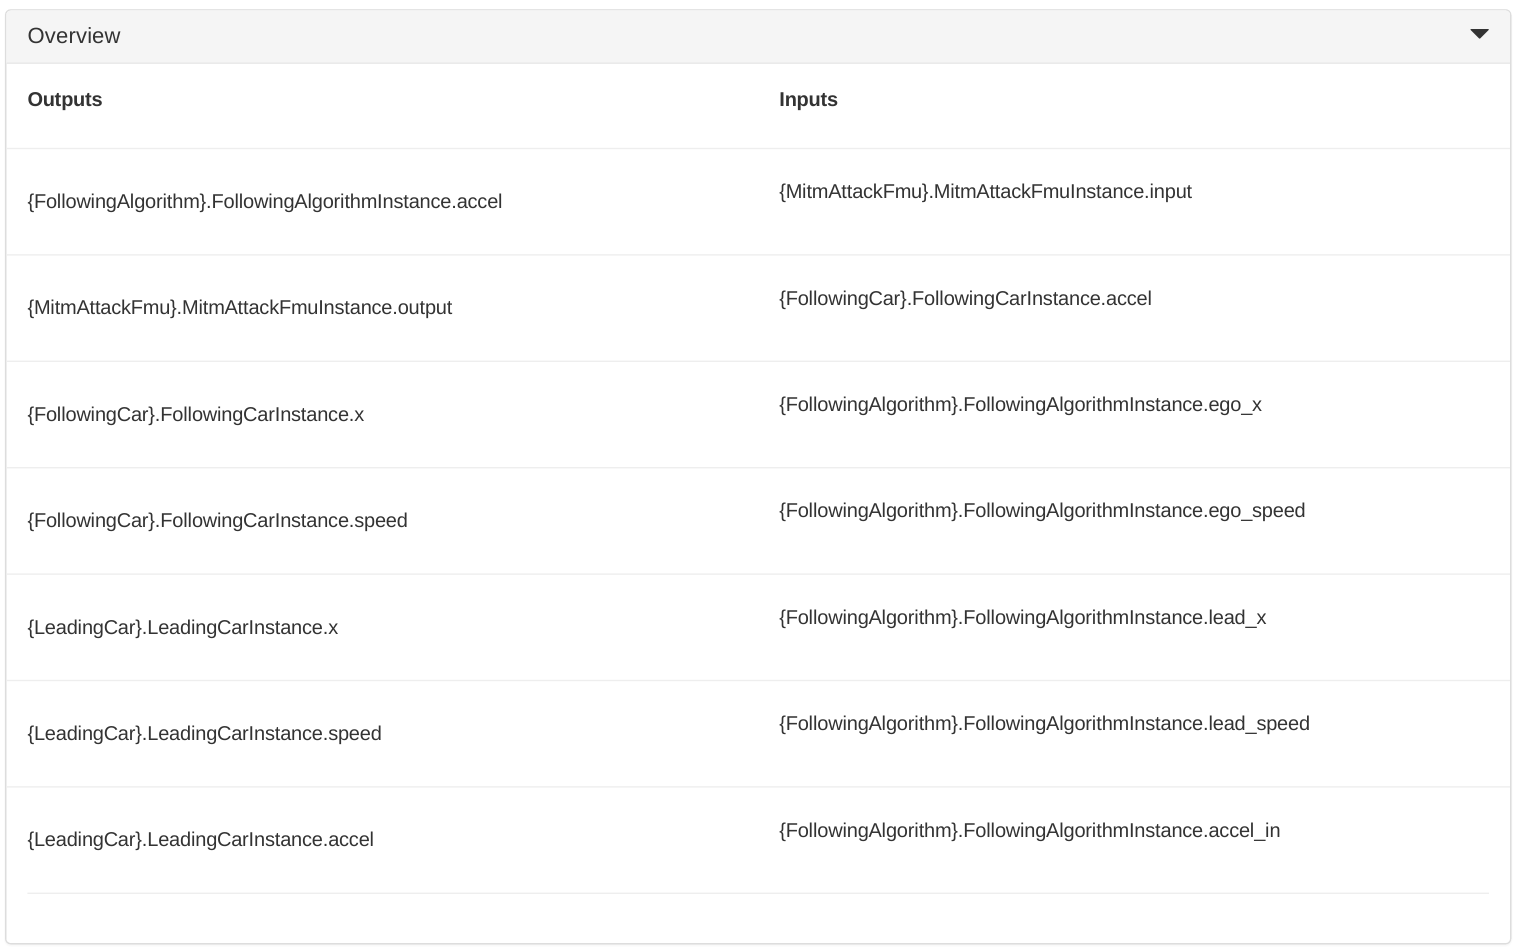
\includegraphics[width=\textwidth]{img/OverviewAccelMulti.png}
	\caption{Multi-Model Overview dell'attacco all'accelerazione (caso attacco multiplo)}
\end{figure}

\subsection{Attacco alla Posizione }
A differenza dello schema presentato nel VanillaCase, viene ora aggiunta una ulteriore FMU situata fra "FMU of the following car" e "FMU of the following algorithm" già presenti. La nuova FMU implementa con strategia \textit{Man-in-the-Middle} un attacco di tipo data alteration sulla posizione passata tra la Following Car e il Following Algorithm. Fare riferimento alla sezione 3.5 per dettagli sul comportamento dell'attacco.

\begin{figure}[H]
	\centering
	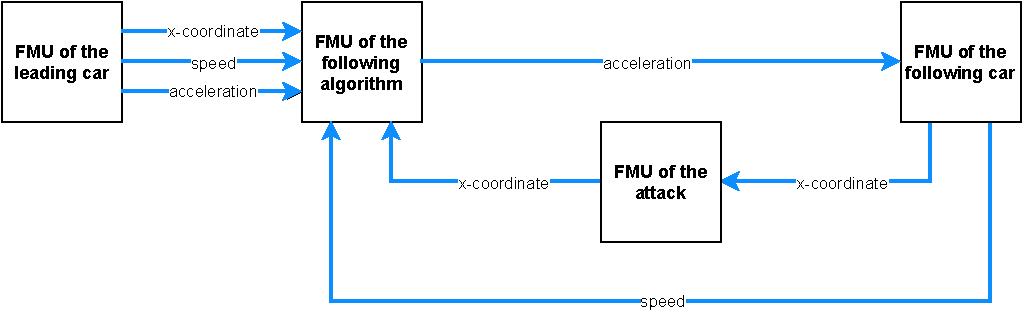
\includegraphics{img/XAttackSchema.pdf}
	\caption{Multi-Model schema dell'Attacco alla Posizione}
\end{figure}

In figura 7 e 8 viene rappresentata l'overview del relativo Multi-Model sviluppato con il tool INTO-CPS. 


\begin{figure}[H]
	\centering
	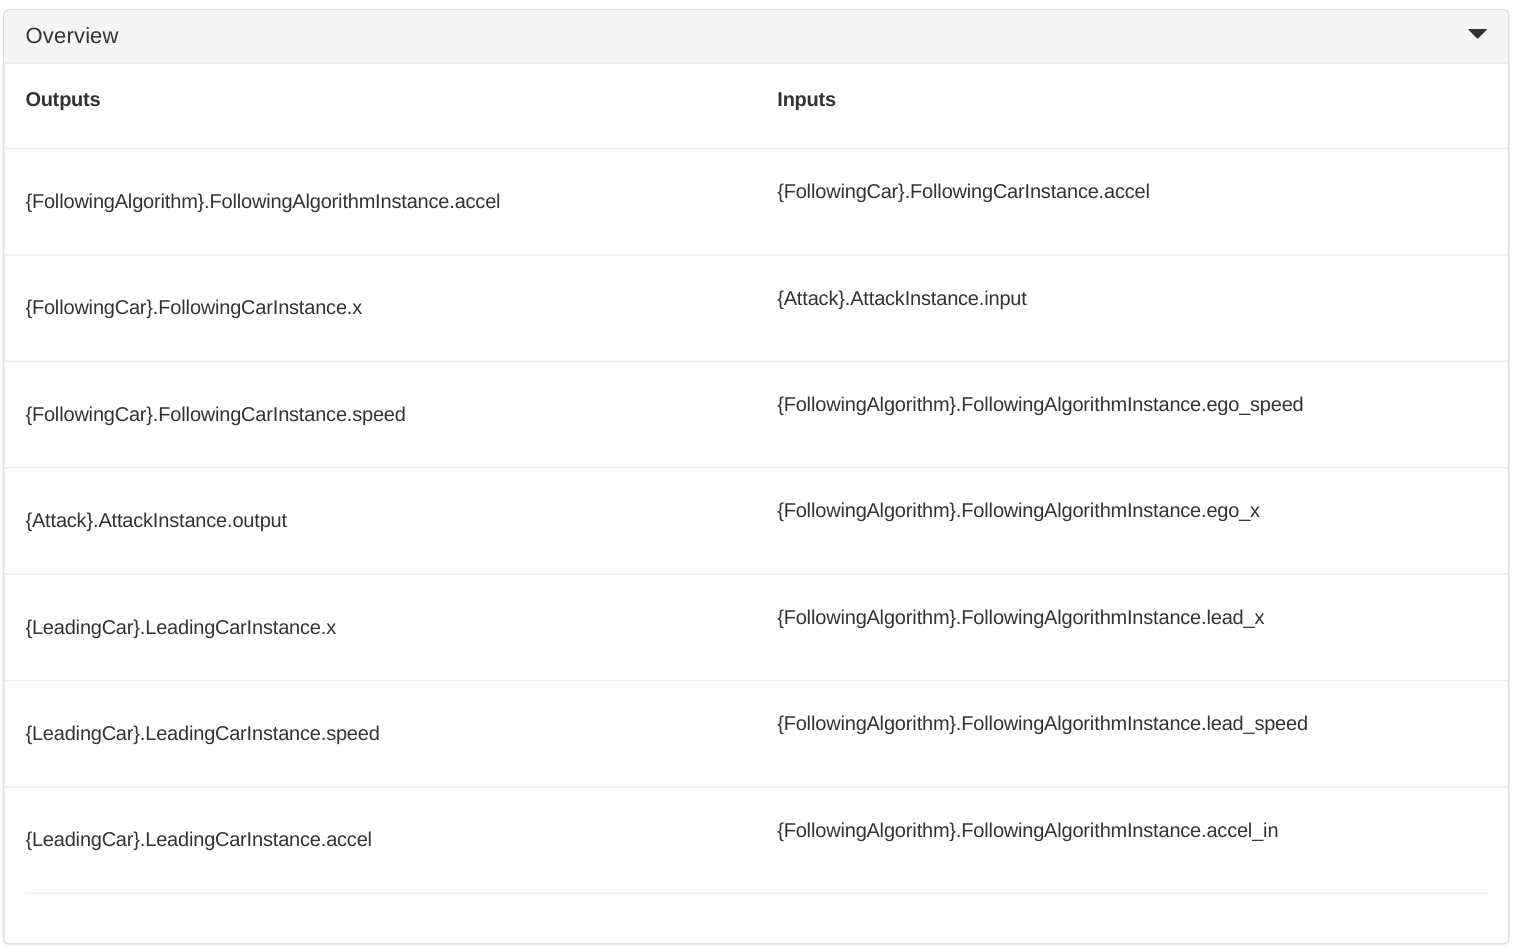
\includegraphics[width=\textwidth]{img/OverviewXSingle.png}
	\caption{Multi-Model Overview dell'attacco alla posizione (caso attacco semplice)}
\end{figure}
\begin{figure}[H]
	\centering
	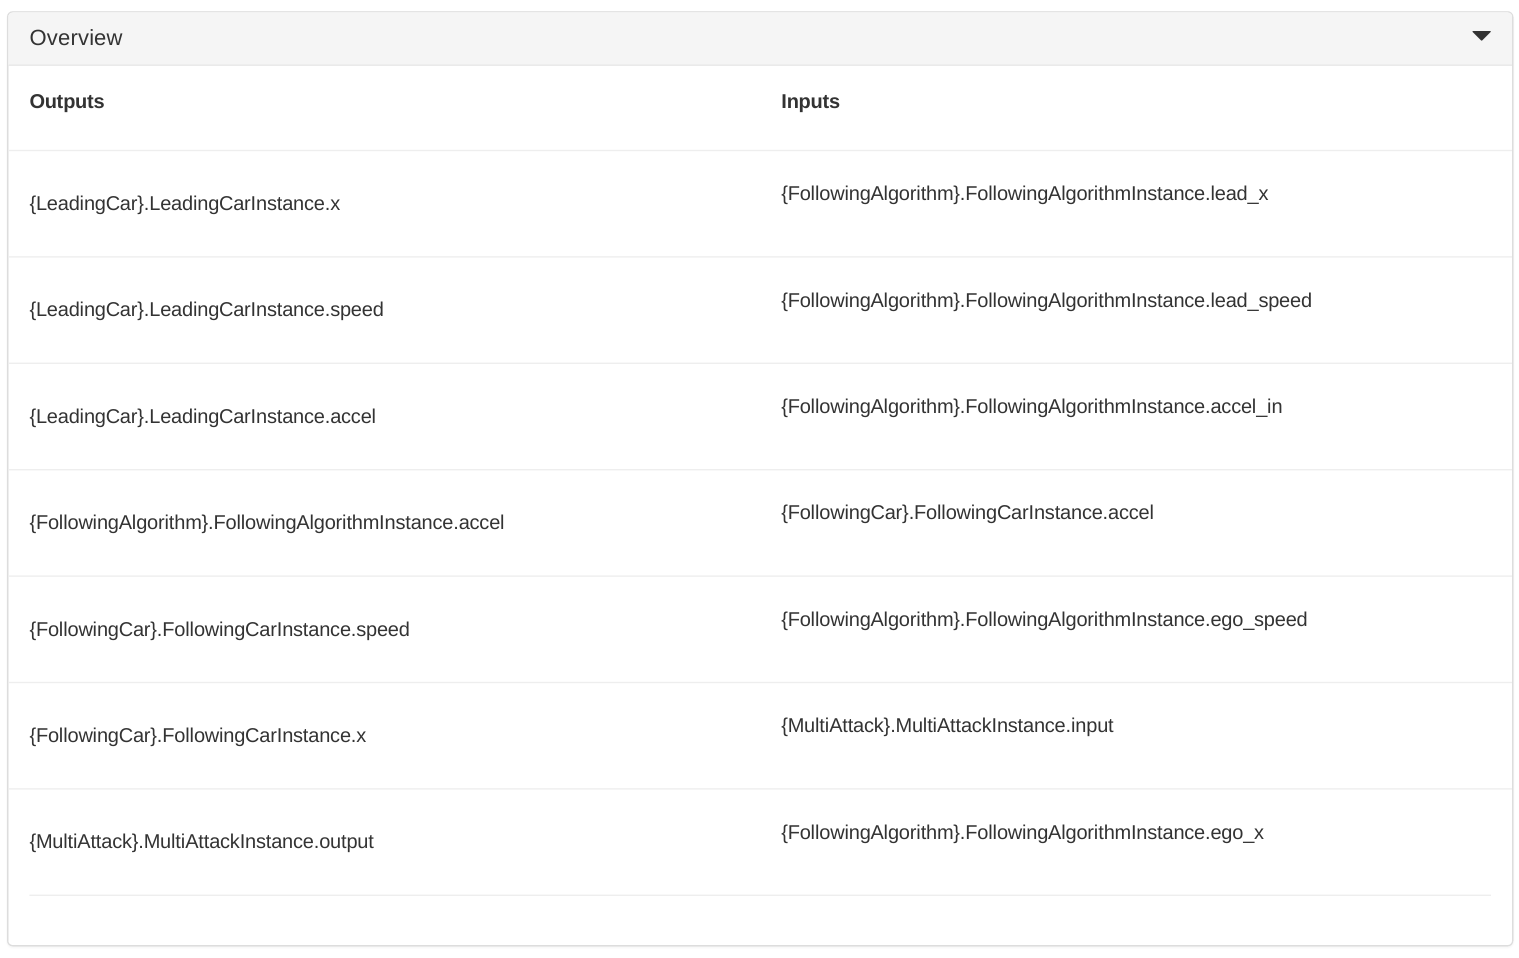
\includegraphics[width=\textwidth]{img/OverviewXMulti.png}
	\caption{Multi-Model Overview dell'attacco alla posizione (caso attacco multiplo)}
\end{figure}

\subsection{Configurazione in Comune}
La configurazione delle seguenti FMU verrà applicata per tutte le simulazioni che verranno effettuate.
\begin{itemize}
	\item \textbf{LeadingCar}:
	\begin{itemize}
		\item Posizione iniziale \textbf{x0}: 50m
		\item Velocità iniziale \textbf{v0}: 0m/s
	\end{itemize}
	
	\item \textbf{FollowingAlgorithm}:
	\begin{itemize}
		\item \textbf{c1}: 0.5
		\item \textbf{eps}: 1
		\item \textbf{omega\_n}: 0.2
	\end{itemize}
	
	
	\item \textbf{FollowingCar}:
	\begin{itemize}
		\item Posizione iniziale \textbf{x0}: 0m
		\item Velocità iniziale \textbf{v0}: 0m/s
	\end{itemize}
\end{itemize}

\subsection{Comportamento degli Attacchi}
L'FMU che verrà utilizzata negli attacchi MITM presenterà due implementazioni diverse:
\begin{itemize}
\item \textbf{Attacco Semplice}: l'attacco consiste nel modificare l'input dell'FMU di attacco con il valore del parametro \textbf{attack\_value} dall'istante temporale \textbf{attack\_time} fino al termine della simulazione. Tale valore viene restituito in output dall'FMU di attacco. Tale FMU è implementata tramite il file Attack\_fmu.fmu. Sono pertanto riportati due estratti di codice implementativo della suddetta FMU: nel primo estratto vi è rappresentata la struttura che rappresenta lo stato dell'fmu. Nel secondo caso è rappresentata l'evoluzione dello stato ad ogni step\_size.

\begin{lstlisting}[language=C++]
	//in sources/misraC/Attack_fmu.h
	typedef struct { 
		Mode mode;
		Mode previous_mode;
		float64_t attack_time; //-- real
		float64_t attack_value; //-- real
		float64_t input; //-- real
		float64_t output; //-- real
		float64_t step_size; //-- real
		float64_t time; //-- real
	} State;

\end{lstlisting}
\begin{lstlisting}[language=C++]
	//in misraC/Attack_fmu.c
	State* tick(State* st) {
		// assert( per_tick(st) );
		if (st->mode == X1 && ( st->time < st->attack_time )) {
			#ifdef DBG
			_dbg_print_condition("st->mode == X1 && ( st->time < st->attack_time )");
			#endif
			leave(X1, st);
			st->output = st->input;
			st->time = st->time + st->step_size;
			enter(X1, st);
		} else if (st->mode == X1 && ( st->time >= st->attack_time )) {
			#ifdef DBG
			_dbg_print_condition("st->mode == X1 && ( st->time >= st->attack_time )");
			#endif
			leave(X1, st);
			st->output = st->attack_value;
			st->time = st->time + st->step_size;
			enter(X1, st);
		}
		#ifdef DBG
		_dbg_print_state(st);
		#endif
		return st;
	}
	
\end{lstlisting}

\item \textbf{Attacco Multi-step}: l'attacco consiste nel modificare l'input dell'FMU di attacco con il valore del parametro \textbf{attack\_value} per un tempo pari a \textbf{attack\_duration}, ripetuto \textbf{attack\_occurrencies} volte e separato nel tempo da \textbf{attack\_distance} secondi. Tale valore viene restituito in output dall'FMU di attacco. L'attacco inizierà dall'istante temporale \textbf{attack\_time}. Tale FMU è implementata tramite il file MultiStep\_MultiAttacks\_Fmu.fmu. Sono mostrati pertanto due estratti della relativa documentazione: nel primo estratto viene rappresentata la differenza in termini di stato dell'Fmu rispetto al caso precedente. Nel secondo estratto viene rappresentata l'evoluzione dello stato dell'Fmu.

\end{itemize}

\begin{lstlisting}[language=C++]
	
	//in sources/misraC/Attack_fmu.h
	//Sono sottolineate le modifiche alla struttura dello stato
	typedef struct { 
		...
		float64_t attack_duration; //-- real
		uint64_t attack_occurrences; //-- integer
		float64_t attack_distance; //-- real
	} State;
	
\end{lstlisting}
\begin{lstlisting}[language=C++]
	//in misraC/Attack_fmu.c
	//Sono sottolineate le modifiche alla tick function
	bool under_attack(State* st){
		float64_t attack_time_i;
		if(st->time >= st->attack_time) {
			for (unsigned int i = 0; i < st->attack_occurrences; ++i){
				//individuo l'inizio di ogni intervallo di attacco
				attack_time_i = st->attack_time + (st->attack_duration + st->attack_distance)*i;
				//vedo se sono nel mezzo di un intervallo
				if(st->time >= attack_time_i && st->time <= attack_time_i + st->attack_duration)
				return true;
			}
		}
		return false;
	}
	
	State* tick(State* st) {
		// assert( per_tick(st) );
		if (st->mode == X1 && !under_attack(st)) {
			#ifdef DBG
			_dbg_print_condition("st->mode == X1 && ( st->time < st->attack_time )");
			#endif
			leave(X1, st);
			st->output = st->input;
			st->time = st->time + st->step_size;
			enter(X1, st);
		} else if (st->mode == X1 && under_attack(st)) {
			#ifdef DBG
			_dbg_print_condition("st->mode == X1 && ( st->time >= st->attack_time )");
			#endif
			leave(X1, st);
			st->output = st->attack_value;
			st->time = st->time + st->step_size;
			enter(X1, st);
		}
		#ifdef DBG
		_dbg_print_state(st);
		#endif
		return st;
	}
\end{lstlisting}